% this file is called up by thesis.tex
% content in this file will be fed into the main document

\chapter{Player Engine Design} % top level followed by section, subsection

\section{Overview}
This chapter describes the design, usage and programming interface. My focus 
will be on communication between the GUI component and the player engine, and 
the ``service'' player engine provides. In the implementation, the player 
engine is executed in an independent thread, the perfermer thread. The 
message queue is similar to unix-style ``pipe'' between two programs. The 
player engine is periodically invoked up by an external timer to 
execute a predefined task including checking the message queue and handling 
pending requests. The external timer is set to 10ms, enabling user 
input to be immediatelly passed to the player engine through message queue and 
processed. Since messages are buffered slightly ahead and accurately timed 
using timestamps, the latency is small and can be ignored.

\begin{figure}[H]
\center{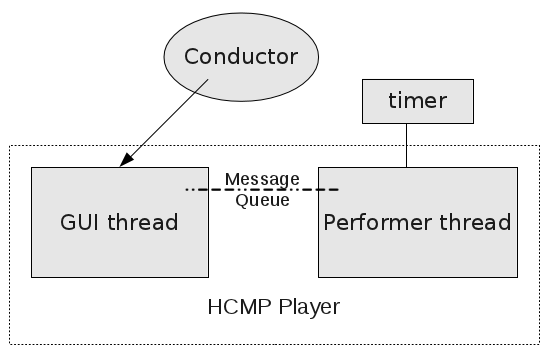
\includegraphics[width=0.55\linewidth]{3/3.png}}
\caption{GUI Thread and Performer Thread}
\label{fig:speciation}
\end{figure}

The player engine serves two major purposes. First it receives
messages from the GUI component and processes them. The second purpose is to 
schedule and play MIDI events at the desire time, and if needed, to
reschedule those scheduled events. In concolusion, the design of the player 
engine is divided into two parts: communication and synchronization. 
Communication refers to the way the player engine and GUI work together. 
Synchronization refers to media synchroization, which involves scheduling 
MIDI notes and the response to changes in tempo. 

\section{Communication}

Figure 3.2 illustrates communication between the GUI component and the player 
engine. In this figure, the GUI component receives a request and works as the 
``front-end'' part of the HCMP Player, and the player engine works as the 
``back-end'' acting on the request. 

In stand-alone mode, the GUI component 
receives requests from user-generated events of clicking a button or adjusting 
the slider bar. These events are captured by the GUI component, processed and 
then passed to player engine. In network mode, the request is captured through 
the network interface. The GUI receives the request when it first arrives 
from the network. The player engine does not differentiate between requests 
originating from user input and processed through the GUI and requests 
originating from a remote server and processed through the GUI component. 
A unified API between the GUI component and the player engine is defined to
clearly illustrate the responsiblity boundary of each module. Note that the 
API between GUI component and the player engine is different from the network API. 
The former is an internal API between two modules, the latter is defined to 
coordinate between a remote server and multiple instances of HCMP players.

\begin{figure}[H]
\center{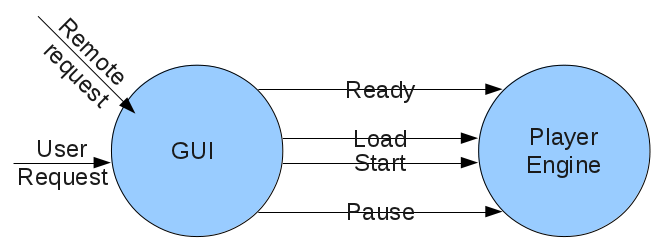
\includegraphics[width=0.7\linewidth]{3/4.png}}
\caption{GUI and Player Engine}
\label{fig:speciation}
\end{figure}

\subsection{Graphical User Interface Thread}

Table 3.2 lists the buttons shown on the GUI component. Each button will send
the request listed when clicked by a user and in stand-alone mode.

\begin{table}[htdp]
\centering
\begin{tabular}{|l||*{2}{c|}}\hline
GUI component & Send Request \\ \hline
load button & load\_file \\\hline
play button & play\\\hline
pause button & pause \\\hline
stop button & stop \\\hline
network button & send\_con\_req \\\hline
tempo slider & change\_tempo \\\hline
volume slider & change\_volume \\\hline
\end{tabular}

\caption[GUI Component and its Request]{GUI Component \& Request}
\label{latexin_genes}
\end{table}

\subsection{State Transition Diagram}

Table 3.2 and 3.3 are state transition diagrams for player engine. The leftmost 
column lists state and the top row list methods. Each (column, row) pair in the 
table indicates what the player engine state will change to given the initial 
state (left column) and method invoked (top row). 

The player engine only receives and accepts control messages from the GUI 
component. It immediately processes the message upon receiving it. The 
implementation uses a hash-like data structure to store the invoking
methods. The key is a pair of current state and request, the value is the method
which changes the current state to a new state. It is similar to the previous 
state transition diagram. When the player engine thread is 
created, it also initializes a timer to periodically invoke itself. 

%Note that to avoid dropping request problem from happening, 
%we need make sure that all the routinues can be executed and completed within 
%bounded time.

\begin{table}[htdp]
\centering
\begin{tabular}{|l||*{6}{c|}}\hline
\backslashbox{State}{Method}
&\makebox load & play & pause & stop \\\hline\hline
uninitialize & ready & undefine & undefine & undefine \\\hline
ready & ready & pause & ready & undefine \\\hline
playing & ready & playing & pause & ready \\\hline
pause & ready & playing & pause & ready  \\\hline
network& con\_ready & undefine & con\_suspend& undefine\\\hline 
\end{tabular}

\caption[Player Engine State Transition Diagram]{Player Engine State Transition Diagram}
\label{latexin_genes}
\end{table}

\begin{table}[htdp]
\centering
\begin{tabular}{|l||*{2}{c|}}\hline
\backslashbox{State}{Method}
&\makebox change\_tempo & change\_volume\\\hline\hline
uninitialize &  undefine & undefine \\\hline
ready & undefine & undefine \\\hline
playing & apply\_change & apply\_change \\\hline
pause  & apply\_change & apply\_change \\\hline
network & undefine & undefine \\\hline 
\end{tabular}
\caption[Player Engine State Transition Diagram]{Player Engine State Transition Diagram}
\label{latexin_genes}
\end{table}
\section{Media Synchronization}

To accurately schedule the MIDI note and apply tempo changes, the player 
engine requires two schedulers, a real-time scheduler and a virtual-time 
scheduler. 

A computation will perform an action needed at the present time,
then schedule the next action. The role of the real-time scheduler is to keep 
track of all pending actions and to invoke them at the proper time. This 
eliminates the need for players to wait, poll or otherwise waste computer 
cycles to ensure that their next computation is performed on time. The 
virtual-time scheduler works at the beat level. Once tempo is changed, either 
due to an internal parameter of a MIDI file or an external signal, there is 
no need to reschedule everything. This is a huge advantage. By using the 
virtual-time scheduler, we only need to rearrange a limited number of MIDI 
notes.

\subsection{Tempo Prediction}
Most popular music forms have a common structure of beats and measures across
all instruments. Thus, time is measured in beats. The basis for synchronization 
in the HCMP Project is a shared notion of the current beat and the current 
tempo. Beats are represented by a floating point number, they are continuous 
rather than integers or messages such as in MIDI clock messages. Rather than 
update the beat number at frequent intervals, we use a linear mapping from time to
beat. This mapping is conveniently expressed using three parameters 
($b_0$, $t_0$, $s$):
\begin{equation}
b = b_0 + (t - t_0) * s 
\end{equation}

where tempo $s$ is expressed in beats per second, at some time in the past beat $b_0$
occurred at time $t_0$, the current time is $t$, and the current beat is $b$.

\begin{figure}[H]
\center{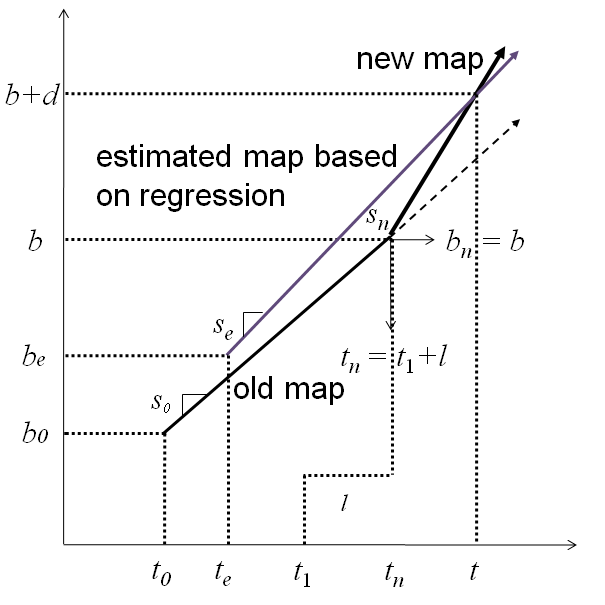
\includegraphics[width=0.5\linewidth]{3/2.png}}
\caption{Linear Mapping Tempo Prediction \cite{Dawen:ISMIR2011}}
\label{fig:speciation}
\end{figure}

One advantage of this approach is that there is almost no latency.
One can send ($t_0$, $b_0$, $s$) to another computer or process and the 
mapping will remain valid regardless of the transmission latency. 
When parameters change, there can be a small different in the current 
time among various processes, but this should be small given that tempo 
is normally steady.

Media players schedule computation to affect the output at specific beat
times. For example, an audio player may begin a sample playback at beat 3, or a
MIDI player may send a note-on message at beat 5. The current beat time $b$ in 
equation 3.1 refers to the beat position of media which is being played.
The audio output buffer contains 0.01s of audio, so then computation associated 
with beat $b$ should be performed 0.01s earlier than $b$. Thus, given a 
player-specific latency $l$, we need to compute the real time $t$ at which to 
schedule a computation associated
with beat $b$. The following formula is easily derived:

\begin{equation}
t = t_0 + (b - b_0) / s - l
\end{equation}

We simply map the beat position $b$ according to ($b_0$, $t_0$, $s$), and then subtract the
latency $l$ to get the computation time $t$.

Our current scheduelr use a simple method to predict the beat . 
A linear regression over recent taps is used to estimate the
mapping from beat to time. 

Once the tempo and beat phase is established, we can determine an
offset from the arbitrary beat number to the beat number in the score. This might
be determined by a external signal that instructs the system when to begin 
playing. The important point here is that some mechanism estimates a local 
mapping between time and beat position, and this mapping is updated as 
the performance progresses.

\subsection{Scheduling}

Schedulers in the HCMP Player accept requests to perform specific
computations at specific times in the future. The specified time 
can be a ``virtual'' time in units such as beats that are translated to real 
time according to a tempo, as in equation 3.1. All pending events can be 
sorted according to beat time. The player engine accepts the event and 
reads its time-stamp. Only the time of this earliest event needs to be 
recomputed if the tempo changes. With event times computed according to 
equation 3.1, only the earliest pending event needs to change when tempo
changes. This is an important feature of the HCMP Player.

\section{Player Engine Programming Interface}
In this section, I describe the API that GUI uses to communicate with player 
engine. The GUI and player engine communicate with each other using strings.
A typical string message will be 
\texttt{"method\_name;argument1;argument2;argument3"}, each argument is 
separated by a \texttt{";"}
character. When passing in the parameter string, the player engine
uses a split-like function to parse the string and store all elements 
into an array. After parsing the request string, the first element 
(the request name) and the player engine's current state form a pair. 
This pair will be used as an argument for the state transition matrix
to fetch the method to change the current state to a new state.\\
Player control related commands 
\begin{itemize}
  \item \texttt{load - "load;file\_path"}
  \item \texttt{play - "play;void"}  
  \item \texttt{pause - "pause;void"}
  \item \texttt{stop - "stop;void"}
\end{itemize}
Audio control related commands 
\begin{itemize}
  \item \texttt{change\_volume - "change\_volume;track\_num;velocity"}  
  \item \texttt{change\_tempo - "change\_tempo;tempo\_scale\_coefficient"}  
\end{itemize}
Connection mode command (detail define in the following chapter)
\begin{itemize}
  \item \texttt{ini\_connection - "ini\_connection;void"}  
\end{itemize}
